% Options for packages loaded elsewhere
\PassOptionsToPackage{unicode}{hyperref}
\PassOptionsToPackage{hyphens}{url}
\PassOptionsToPackage{dvipsnames,svgnames,x11names}{xcolor}
%
\documentclass[
  12pt,
  a4paper]{article}
\usepackage{amsmath,amssymb}
\usepackage{lmodern}
\usepackage{iftex}
\ifPDFTeX
  \usepackage[T1]{fontenc}
  \usepackage[utf8]{inputenc}
  \usepackage{textcomp} % provide euro and other symbols
\else % if luatex or xetex
  \usepackage{unicode-math}
  \defaultfontfeatures{Scale=MatchLowercase}
  \defaultfontfeatures[\rmfamily]{Ligatures=TeX,Scale=1}
\fi
% Use upquote if available, for straight quotes in verbatim environments
\IfFileExists{upquote.sty}{\usepackage{upquote}}{}
\IfFileExists{microtype.sty}{% use microtype if available
  \usepackage[]{microtype}
  \UseMicrotypeSet[protrusion]{basicmath} % disable protrusion for tt fonts
}{}
\makeatletter
\@ifundefined{KOMAClassName}{% if non-KOMA class
  \IfFileExists{parskip.sty}{%
    \usepackage{parskip}
  }{% else
    \setlength{\parindent}{0pt}
    \setlength{\parskip}{6pt plus 2pt minus 1pt}}
}{% if KOMA class
  \KOMAoptions{parskip=half}}
\makeatother
\usepackage{xcolor}
\usepackage[margin=0.7in]{geometry}
\usepackage{color}
\usepackage{fancyvrb}
\newcommand{\VerbBar}{|}
\newcommand{\VERB}{\Verb[commandchars=\\\{\}]}
\DefineVerbatimEnvironment{Highlighting}{Verbatim}{commandchars=\\\{\}}
% Add ',fontsize=\small' for more characters per line
\usepackage{framed}
\definecolor{shadecolor}{RGB}{248,248,248}
\newenvironment{Shaded}{\begin{snugshade}}{\end{snugshade}}
\newcommand{\AlertTok}[1]{\textcolor[rgb]{0.94,0.16,0.16}{#1}}
\newcommand{\AnnotationTok}[1]{\textcolor[rgb]{0.56,0.35,0.01}{\textbf{\textit{#1}}}}
\newcommand{\AttributeTok}[1]{\textcolor[rgb]{0.77,0.63,0.00}{#1}}
\newcommand{\BaseNTok}[1]{\textcolor[rgb]{0.00,0.00,0.81}{#1}}
\newcommand{\BuiltInTok}[1]{#1}
\newcommand{\CharTok}[1]{\textcolor[rgb]{0.31,0.60,0.02}{#1}}
\newcommand{\CommentTok}[1]{\textcolor[rgb]{0.56,0.35,0.01}{\textit{#1}}}
\newcommand{\CommentVarTok}[1]{\textcolor[rgb]{0.56,0.35,0.01}{\textbf{\textit{#1}}}}
\newcommand{\ConstantTok}[1]{\textcolor[rgb]{0.00,0.00,0.00}{#1}}
\newcommand{\ControlFlowTok}[1]{\textcolor[rgb]{0.13,0.29,0.53}{\textbf{#1}}}
\newcommand{\DataTypeTok}[1]{\textcolor[rgb]{0.13,0.29,0.53}{#1}}
\newcommand{\DecValTok}[1]{\textcolor[rgb]{0.00,0.00,0.81}{#1}}
\newcommand{\DocumentationTok}[1]{\textcolor[rgb]{0.56,0.35,0.01}{\textbf{\textit{#1}}}}
\newcommand{\ErrorTok}[1]{\textcolor[rgb]{0.64,0.00,0.00}{\textbf{#1}}}
\newcommand{\ExtensionTok}[1]{#1}
\newcommand{\FloatTok}[1]{\textcolor[rgb]{0.00,0.00,0.81}{#1}}
\newcommand{\FunctionTok}[1]{\textcolor[rgb]{0.00,0.00,0.00}{#1}}
\newcommand{\ImportTok}[1]{#1}
\newcommand{\InformationTok}[1]{\textcolor[rgb]{0.56,0.35,0.01}{\textbf{\textit{#1}}}}
\newcommand{\KeywordTok}[1]{\textcolor[rgb]{0.13,0.29,0.53}{\textbf{#1}}}
\newcommand{\NormalTok}[1]{#1}
\newcommand{\OperatorTok}[1]{\textcolor[rgb]{0.81,0.36,0.00}{\textbf{#1}}}
\newcommand{\OtherTok}[1]{\textcolor[rgb]{0.56,0.35,0.01}{#1}}
\newcommand{\PreprocessorTok}[1]{\textcolor[rgb]{0.56,0.35,0.01}{\textit{#1}}}
\newcommand{\RegionMarkerTok}[1]{#1}
\newcommand{\SpecialCharTok}[1]{\textcolor[rgb]{0.00,0.00,0.00}{#1}}
\newcommand{\SpecialStringTok}[1]{\textcolor[rgb]{0.31,0.60,0.02}{#1}}
\newcommand{\StringTok}[1]{\textcolor[rgb]{0.31,0.60,0.02}{#1}}
\newcommand{\VariableTok}[1]{\textcolor[rgb]{0.00,0.00,0.00}{#1}}
\newcommand{\VerbatimStringTok}[1]{\textcolor[rgb]{0.31,0.60,0.02}{#1}}
\newcommand{\WarningTok}[1]{\textcolor[rgb]{0.56,0.35,0.01}{\textbf{\textit{#1}}}}
\usepackage{graphicx}
\makeatletter
\def\maxwidth{\ifdim\Gin@nat@width>\linewidth\linewidth\else\Gin@nat@width\fi}
\def\maxheight{\ifdim\Gin@nat@height>\textheight\textheight\else\Gin@nat@height\fi}
\makeatother
% Scale images if necessary, so that they will not overflow the page
% margins by default, and it is still possible to overwrite the defaults
% using explicit options in \includegraphics[width, height, ...]{}
\setkeys{Gin}{width=\maxwidth,height=\maxheight,keepaspectratio}
% Set default figure placement to htbp
\makeatletter
\def\fps@figure{htbp}
\makeatother
\setlength{\emergencystretch}{3em} % prevent overfull lines
\providecommand{\tightlist}{%
  \setlength{\itemsep}{0pt}\setlength{\parskip}{0pt}}
\setcounter{secnumdepth}{5}
\ifLuaTeX
\usepackage[bidi=basic]{babel}
\else
\usepackage[bidi=default]{babel}
\fi
\babelprovide[main,import]{spanish}
% get rid of language-specific shorthands (see #6817):
\let\LanguageShortHands\languageshorthands
\def\languageshorthands#1{}
\usepackage{sfmath}
\renewcommand*\familydefault{\sfdefault}
\renewcommand{\baselinestretch}{1.2}
\setlength{\parskip}{1em}
\usepackage{xcolor}
\DefineVerbatimEnvironment{Highlighting}{Verbatim}{fontsize=\small, commandchars=\\\{\}}
\AtBeginEnvironment{Verbatim}{\setlength{\lineskip}{0pt}}


% make console-output smaller:
\makeatletter
\def\verbatim{\small\@verbatim \frenchspacing\@vobeyspaces \@xverbatim}
\makeatother


% \setlength{\parskip}{0pt}

\AtBeginEnvironment{verbatim}{\renewcommand{\baselinestretch}{1}}

\setlength{\OuterFrameSep}{0pt}
\makeatletter
\preto{\@verbatim}{\topsep=-10pt \partopsep=5pt \itemsep=0pt}
\makeatother

\usepackage{titlesec}
\titleformat*{\section}{\Large\bfseries}
\titleformat*{\subsection}{\large\bfseries}

\ifLuaTeX
  \usepackage{selnolig}  % disable illegal ligatures
\fi
\usepackage[style=bwl-FU,]{biblatex}
\addbibresource{references.bib}
\IfFileExists{bookmark.sty}{\usepackage{bookmark}}{\usepackage{hyperref}}
\IfFileExists{xurl.sty}{\usepackage{xurl}}{} % add URL line breaks if available
\urlstyle{same} % disable monospaced font for URLs
\hypersetup{
  pdftitle={Simulaciones},
  pdfauthor={Ana Xiangning Pereira Ezquerro},
  pdflang={es},
  colorlinks=true,
  linkcolor={blue},
  filecolor={Maroon},
  citecolor={Blue},
  urlcolor={Blue},
  pdfcreator={LaTeX via pandoc}}

\title{Simulaciones}
\author{Ana Xiangning Pereira Ezquerro}
\date{Versión 26 julio, 2022}

\begin{document}
\maketitle

{
\hypersetup{linkcolor=}
\setcounter{tocdepth}{2}
\tableofcontents
}
\vspace{2em}

En este documento se exponen múltiples simulaciones de la selección
automática de variables con sus respectivos retardos usando una nueva
propuesta. Se mostrarán ejemplos donde la selección automática trabaja
sobre un conjunto de variables de las cuales sólo algunas inciden en la
variable respuesta y con un retardo concreto (aunque siempre menor o
igual a 0). A lo largo de las siguientes secciones se irán complicando
escenarios con la finalidad de analizar cómo se comporta la nueva
propuesta ante datos simulados e inferir a partir de ellos cómo se
comportará en escenarios reales.

\textbf{Nota}: Para generar los datos de las simulaciones se usó el
código \texttt{arima\_simulation.R}, el cual permite generar de forma
pseudo-aleatoria series temporales a partir de un proceso ARIMA. Este
documento no muestra cómo generar las series (para evitar la
aleatoriedad de los resultados), sino que, una vez generadas y
guardadas, se cargan directamente de memoria.

\newpage

\hypertarget{simulaciuxf3n-de-un-modelo-de-regresiuxf3n-dinuxe1mica-con-errores-estacionarios}{%
\section{Simulación de un modelo de regresión dinámica con errores
estacionarios}\label{simulaciuxf3n-de-un-modelo-de-regresiuxf3n-dinuxe1mica-con-errores-estacionarios}}

En esta sección veremos cómo se comporta la función de selección
automática sobre ejemplos muy básicos donde los errores del modelo son
estacionarios:

\[Y_t = \beta_0 + \beta_1 X_{t-r_1}^{(1)} + \beta_2 X_{t-r_2}^{(2)} + \cdots + X_{t-r_p}^{(p)}+ \eta_t, \qquad \eta_t \sim \text{ARMA(p,q)}, \quad r_i \geq 0 \text{ para } i=1,..., p \]

\hypertarget{ejemplo1}{%
\subsection{\texorpdfstring{Modelo donde \(r_i=0\) para
\(i=1,...,p\)}{Modelo donde r\_i=0 para i=1,...,p}}\label{ejemplo1}}

Supongamos un modelo de regresión dinámica de tres variables regresoras
donde todos los retardos son igual a cero. En concreto, nuestro modelo
tendrá la forma:

\begin{equation}\label{eq:ejemplo1}
    Y_t = \beta_0 + \beta_1 X_t^{(1)} + \beta_2 X_t^{(2)} + \beta_3 X_t^{(3)} + \eta_t
\end{equation}

donde:

\begin{itemize}
\tightlist
\item
  \(\eta_t \sim\) ARMA(2,1), por tanto, los errores son estacionarios.
\item
  \(X_t^{(1)} \sim\) ARIMA(2, 1, 3) y su coeficiente \(\beta_1 = 2.8\).
\item
  \(X_t^{(2)} \sim\) ARIMA(1, 1, 2) y su coeficiente
  \(\beta_2 = -1.12\).
\item
  \(X_t^{(3)} \sim\) ARMA(1, 2) y su coeficiente \(\beta_3 = -2.3\).
\item
  El \emph{intercept} es \(\beta_0=0.8\).
\end{itemize}

Supongamos otro conjunto de variables (que siguen también un proceso
ARIMA) que no van a influir en la variable respuesta:

\begin{itemize}
\tightlist
\item
  \(X_t^{(4)} \sim\) ARIMA(1, 0, 3).
\item
  \(X_t^{(5)} \sim\) ARIMA(2, 1, 2).
\item
  \(X_t^{(6)} \sim\) ARIMA(2, 1, 1).
\end{itemize}

\begin{Shaded}
\begin{Highlighting}[]
\CommentTok{\# Cargamos los datos sobre las variables regresoras}
\FunctionTok{load}\NormalTok{(}\AttributeTok{file=}\StringTok{\textquotesingle{}simulations/X1 \textasciitilde{} ARIMA(2,1,3).RData\textquotesingle{}}\NormalTok{)        }\CommentTok{\# X1}
\FunctionTok{load}\NormalTok{(}\AttributeTok{file=}\StringTok{\textquotesingle{}simulations/X2 \textasciitilde{} ARIMA(1,1,2).RData\textquotesingle{}}\NormalTok{)        }\CommentTok{\# X2}
\FunctionTok{load}\NormalTok{(}\AttributeTok{file=}\StringTok{\textquotesingle{}simulations/X3 \textasciitilde{} ARIMA(1,0,2).RData\textquotesingle{}}\NormalTok{)        }\CommentTok{\# X3}
\FunctionTok{load}\NormalTok{(}\AttributeTok{file=}\StringTok{\textquotesingle{}simulations/residuals \textasciitilde{} ARIMA(2,0,1).RData\textquotesingle{}}\NormalTok{) }\CommentTok{\# residuos}

\CommentTok{\# Cargamos las variables independientes}
\FunctionTok{load}\NormalTok{(}\AttributeTok{file=}\StringTok{\textquotesingle{}simulations/X4 \textasciitilde{} ARIMA(1,0,3).RData\textquotesingle{}}\NormalTok{)        }\CommentTok{\# X4}
\FunctionTok{load}\NormalTok{(}\AttributeTok{file=}\StringTok{\textquotesingle{}simulations/X5 \textasciitilde{} ARIMA(2,1,2).RData\textquotesingle{}}\NormalTok{)        }\CommentTok{\# X5}
\FunctionTok{load}\NormalTok{(}\AttributeTok{file=}\StringTok{\textquotesingle{}simulations/X6 \textasciitilde{} ARIMA(2,1,1).RData\textquotesingle{}}\NormalTok{)        }\CommentTok{\# X6}
\end{Highlighting}
\end{Shaded}

Se puede realizar una comprobación de que estas series siguen los
procesos ARIMA mencionados. Para chequearlo, consulte el
\protect\hyperlink{apendice}{apéndice} del documento.

\textbf{Selección de variables y ajuste del modelo}: Creamos el modelo y
comprobamos la solución final de la función
\texttt{auto.fit.arima.regression()}.

\begin{Shaded}
\begin{Highlighting}[]
\NormalTok{beta0 }\OtherTok{\textless{}{-}} \FloatTok{0.8}\NormalTok{; beta1 }\OtherTok{\textless{}{-}} \FloatTok{2.8}\NormalTok{; beta2 }\OtherTok{\textless{}{-}} \SpecialCharTok{{-}}\FloatTok{1.12}\NormalTok{; beta3 }\OtherTok{\textless{}{-}} \SpecialCharTok{{-}}\FloatTok{2.3}
\NormalTok{Y }\OtherTok{\textless{}{-}}\NormalTok{ beta0 }\SpecialCharTok{+}\NormalTok{ beta1 }\SpecialCharTok{*}\NormalTok{ X1}\SpecialCharTok{$}\NormalTok{X }\SpecialCharTok{+}\NormalTok{ beta2 }\SpecialCharTok{*}\NormalTok{ X2}\SpecialCharTok{$}\NormalTok{X }\SpecialCharTok{+}\NormalTok{ beta3 }\SpecialCharTok{*}\NormalTok{ X3}\SpecialCharTok{$}\NormalTok{X }\SpecialCharTok{+}\NormalTok{ residuals}\SpecialCharTok{$}\NormalTok{X}
\NormalTok{regresoras }\OtherTok{\textless{}{-}} \FunctionTok{cbind}\NormalTok{(}\AttributeTok{X1=}\NormalTok{X1}\SpecialCharTok{$}\NormalTok{X, }\AttributeTok{X2=}\NormalTok{X2}\SpecialCharTok{$}\NormalTok{X, }\AttributeTok{X3=}\NormalTok{X3}\SpecialCharTok{$}\NormalTok{X, }\AttributeTok{X4=}\NormalTok{X4}\SpecialCharTok{$}\NormalTok{X, }\AttributeTok{X5=}\NormalTok{X5}\SpecialCharTok{$}\NormalTok{X, }\AttributeTok{X6=}\NormalTok{X6}\SpecialCharTok{$}\NormalTok{X)}
\NormalTok{ajuste }\OtherTok{\textless{}{-}} \FunctionTok{auto.fit.arima.regression}\NormalTok{(Y, regresoras, }\AttributeTok{show\_info=}\NormalTok{T)}
\end{Highlighting}
\end{Shaded}

\begin{verbatim}
Se ha probado con la variable X1 [ic=-1135.19120552446, lag=0]
Se ha probado con la variable X2 [ic=-286.986760465024, lag=0]
Se ha probado con la variable X3 [ic=-640.026014781463, lag=0]
No se ha podido encontrar un retardo significativo para X4
No se ha podido encontrar un retardo significativo para X5
Se ha probado con la variable X6 [ic=-186.816241878495, lag=0]
Se ha añadido la variable regresora X1 [aicc=-1135.19120552446, lag=0]
Series: serie 
Regression with ARIMA(4,1,1) errors 

Coefficients:
         ar1     ar2      ar3      ar4      ma1    xreg
      0.3013  0.2546  -0.1522  -0.0784  -0.9035  2.7997
s.e.  0.0378  0.0342   0.0335   0.0347   0.0218  0.0485

sigma^2 = 0.0184:  log likelihood = 574.65
AIC=-1135.31   AICc=-1135.19   BIC=-1101.03
--------------------------------------------------------------------------------------
Se ha probado con la variable X2 [ic=-1396.16397504914, lag=0]
Se ha probado con la variable X3 [ic=-2213.72165014961, lag=0]
No se ha podido encontrar un retardo significativo para X4
No se ha podido encontrar un retardo significativo para X5
No se ha podido encontrar un retardo significativo para X6
Se ha añadido la variable regresora X3 [aicc=-2213.72165014961, lag=0]
Series: serie 
Regression with ARIMA(0,1,3) errors 

Coefficients:
          ma1  ma2      ma3      X1       X3
      -0.5907    0  -0.1460  2.7962  -2.2890
s.e.   0.0274    0   0.0269  0.0350   0.0505

sigma^2 = 0.006201:  log likelihood = 1111.89
AIC=-2213.78   AICc=-2213.72   BIC=-2189.3
--------------------------------------------------------------------------------------
Se ha probado con la variable X2 [ic=-3163.18780840121, lag=0]
No se ha podido encontrar un retardo significativo para X4
No se ha podido encontrar un retardo significativo para X5
Se ha probado con la variable X6 [ic=-2212.54498022128, lag=-3]
Se ha añadido la variable regresora X2 [aicc=-3163.18780840121, lag=0]
Series: serie 
Regression with ARIMA(2,0,1) errors 

Coefficients:
          ar1     ar2     ma1  intercept      X1       X3       X2
      -0.1989  0.4054  0.4443     0.8056  2.7982  -2.2719  -1.1084
s.e.   0.0702  0.0302  0.0746     0.0034  0.0092   0.0320   0.0108

sigma^2 = 0.002375:  log likelihood = 1589.67
AIC=-3163.33   AICc=-3163.19   BIC=-3124.15
--------------------------------------------------------------------------------------
No se ha podido encontrar un retardo significativo para X4
Se ha probado con la variable X5 [ic=-3161.16122909997, lag=-8]
No se ha podido encontrar un retardo significativo para X6
No se añaden más variables
--------------------------------------------------------------------------------------
|                Histórico de variables añadidas al modelo (ndiff=0)                 |
--------------------------------------------------------------------------------------
 var lag                ic
  X1   0 -1135.19120552446
  X3   0 -2213.72165014961
  X2   0 -3163.18780840121
--------------------------------------------------------------------------------------
Series: serie 
Regression with ARIMA(2,0,1) errors 

Coefficients:
          ar1     ar2     ma1  intercept      X1       X3       X2
      -0.1989  0.4054  0.4443     0.8056  2.7982  -2.2719  -1.1084
s.e.   0.0702  0.0302  0.0746     0.0034  0.0092   0.0320   0.0108

sigma^2 = 0.002375:  log likelihood = 1589.67
AIC=-3163.33   AICc=-3163.19   BIC=-3124.15
\end{verbatim}

En el \emph{output} de la función vemos cuál ha sido el proceso de
selección de variables regresoras:

\begin{enumerate}
\def\labelenumi{\arabic{enumi}.}
\tightlist
\item
  En la primera iteración se añade la variable \(X_t^{(1)}\) con retardo
  nulo (algo que es correcto teniendo en cuenta cómo se ha creado el
  modelo en \ref{eq:ejemplo1}) y obteniendo un AICc=-1135.19120552446.
\item
  En la segunda iteración se introduce la variable \(X_t^{(3)}\) con un
  retardo nulo y mejorando el AICc del modelo anterior (que sólo contaba
  con la variable \(X_t^{(1)}\)) con un AICc=-2213.72165014961.
\item
  En la tercera iteración se añade la variable \(X_t^{(2)}\) con retardo
  nulo y mejorando el criterio de información del modelo anterior (que
  tenía las variables \(X_t^{(1)}\) y \(X_t^{(1)}\)) con un
  AICc=-3163.18780840121.
\item
  En la siguiente iteración no se encuentran correlaciones
  significativas con ningún retardo para las variables \(X_t^{(4)}\) y
  \(X_t^{(6)}\), por lo que éstas no se pueden añadir al modelo. Para la
  varialbe \(X_t^{(5)}\), se encuentra un retardo significativo en
  \(k=-8\), pero no se mejora el AICc del modelo anterior (con las tres
  variables regresoras), por lo que se detiene el bucle para añadir
  variables.
\end{enumerate}

Como el modelo resultante de haber añadido de forma iterativa todas las
variables tiene errores estacionarios (siguen un ARIMA(2,0,1), lo que
coincide con la simulación realizada), se considera como modelo válido
para definir la relación entre la variable respuesta \(Y\) y el conjunto
de variables regresoras seleccionadas (\(X_t^{(1)}\), \(X_t^{(2)}\) y
\(X_t^{(3)}\)). Podemos observar cómo el valor del \emph{intercept} y de
los coeficientes de regresión se aproximan bastante a los coeficientes
seleccionados al construir de forma artificial la variable regresora
\(Y\) en @ref(eq:ejemplo1).

\textbf{Predicción}: Finalmente realizamos las predicciones puntuales:

\begin{Shaded}
\begin{Highlighting}[]
\NormalTok{preds }\OtherTok{\textless{}{-}} \FunctionTok{forecast\_model}\NormalTok{(Y, regresoras, ajuste, }\AttributeTok{h=}\DecValTok{10}\NormalTok{, }\AttributeTok{mode=}\StringTok{\textquotesingle{}bootstrap\textquotesingle{}}\NormalTok{)}
\FunctionTok{display}\NormalTok{(}\FunctionTok{plot\_forecast}\NormalTok{(preds, }\AttributeTok{rang=}\FunctionTok{c}\NormalTok{(}\DecValTok{950}\NormalTok{, }\DecValTok{1009}\NormalTok{)), }\AttributeTok{name=}\StringTok{\textquotesingle{}ejemplo1\textquotesingle{}}\NormalTok{)}
\end{Highlighting}
\end{Shaded}

\begin{center}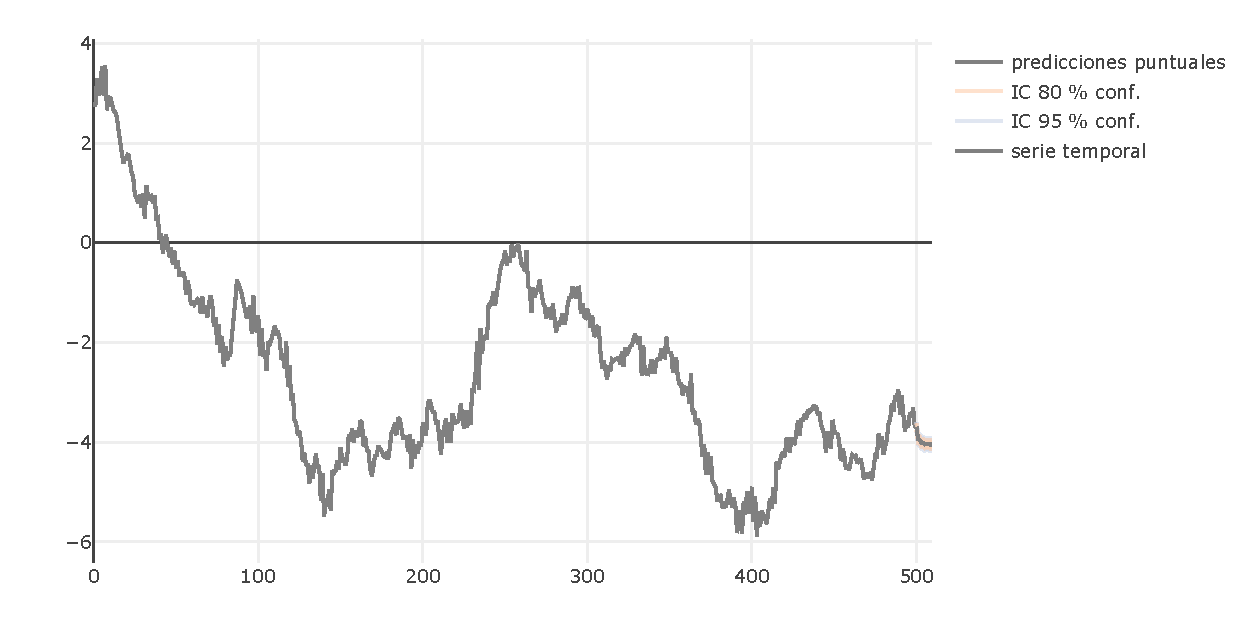
\includegraphics{figures/ejemplo1} \end{center}

\hypertarget{ejemplo2}{%
\subsection{\texorpdfstring{Modelo donde \(r_i\geq 0\) para
\(i=1,...,p\)}{Modelo donde r\_i\textbackslash geq 0 para i=1,...,p}}\label{ejemplo2}}

Supongamos un modelo de regresión dinámica parecido al del
\protect\hyperlink{ejemplo1}{primer ejemplo}, utilizando las mismas
variables, pero donde los retardos sean menores o iguales a 0 (que haya
``variedad'' en los retardos).

\begin{equation}\label{eq:ejemplo2}
    Y_t = \beta_0 + \beta_1 X_{t-r_1}^{(1)} + \beta_2 X_{t-r_2}^{(2)} + \beta_3 X_{t-r_3}^{(3)} + \eta_t
\end{equation}

donde:

\begin{itemize}
\tightlist
\item
  \(\eta_t \sim\) ARMA(2, 1).
\item
  \(X_t^{(1)} \sim\) ARIMA(2, 1, 3) y su retardo \(r_1=2\).
\item
  \(X_t^{(2)} \sim\) ARMA(1, 1, 2) y su retardo \(r_2=0\).
\item
  \(X_t^{(3)} \sim\) ARMA(1, 0, 2) y su retardo \(r_3=3\).
\end{itemize}

\begin{Shaded}
\begin{Highlighting}[]
\CommentTok{\# Construimos el modelo }
\NormalTok{beta0 }\OtherTok{\textless{}{-}} \SpecialCharTok{{-}}\FloatTok{0.6}\NormalTok{; beta1 }\OtherTok{\textless{}{-}} \FloatTok{1.7}\NormalTok{; beta2 }\OtherTok{\textless{}{-}} \SpecialCharTok{{-}}\FloatTok{2.2}\NormalTok{; beta3 }\OtherTok{\textless{}{-}} \FloatTok{1.3}
\NormalTok{r1 }\OtherTok{\textless{}{-}} \DecValTok{2}\NormalTok{; r3 }\OtherTok{\textless{}{-}} \DecValTok{3}
\NormalTok{Y }\OtherTok{\textless{}{-}}\NormalTok{ beta0 }\SpecialCharTok{+}\NormalTok{ beta1 }\SpecialCharTok{*} \FunctionTok{lag}\NormalTok{(X1}\SpecialCharTok{$}\NormalTok{X, }\SpecialCharTok{{-}}\NormalTok{r1) }\SpecialCharTok{+}\NormalTok{ beta2 }\SpecialCharTok{*}\NormalTok{ X2}\SpecialCharTok{$}\NormalTok{X }\SpecialCharTok{+}\NormalTok{ beta3 }\SpecialCharTok{*} \FunctionTok{lag}\NormalTok{(X3}\SpecialCharTok{$}\NormalTok{X, }\SpecialCharTok{{-}}\NormalTok{r3) }\SpecialCharTok{+} 
\NormalTok{    residuals}\SpecialCharTok{$}\NormalTok{X}
\end{Highlighting}
\end{Shaded}

\textbf{Selección de variables y ajuste del modelo}:

\begin{Shaded}
\begin{Highlighting}[]
\NormalTok{regresoras }\OtherTok{\textless{}{-}} \FunctionTok{cbind}\NormalTok{(}\AttributeTok{X1=}\NormalTok{X1}\SpecialCharTok{$}\NormalTok{X, }\AttributeTok{X2=}\NormalTok{X2}\SpecialCharTok{$}\NormalTok{X, }\AttributeTok{X3=}\NormalTok{X3}\SpecialCharTok{$}\NormalTok{X, }\AttributeTok{X4=}\NormalTok{X4}\SpecialCharTok{$}\NormalTok{X, }\AttributeTok{X5=}\NormalTok{X5}\SpecialCharTok{$}\NormalTok{X, }\AttributeTok{X6=}\NormalTok{X6}\SpecialCharTok{$}\NormalTok{X)}
\NormalTok{ajuste }\OtherTok{\textless{}{-}} \FunctionTok{auto.fit.arima.regression}\NormalTok{(Y, regresoras, }\AttributeTok{show\_info=}\NormalTok{T,  }
                                    \AttributeTok{stationary\_method=}\StringTok{\textquotesingle{}adf.test\textquotesingle{}}\NormalTok{)}
\end{Highlighting}
\end{Shaded}

\begin{verbatim}
Se ha probado con la variable X1 [ic=-989.555684098221, lag=-2]
Se ha probado con la variable X2 [ic=-1156.68486061937, lag=0]
Se ha probado con la variable X3 [ic=-802.904991565362, lag=-3]
Se ha probado con la variable X4 [ic=-579.867845971486, lag=-1]
No se ha podido encontrar un retardo significativo para X5
No se ha podido encontrar un retardo significativo para X6
Se ha añadido la variable regresora X2 [aicc=-1156.68486061937, lag=0]
Series: serie 
Regression with ARIMA(4,1,0) errors 

Coefficients:
          ar1      ar2      ar3     ar4     xreg
      -0.4245  -0.3382  -0.1395  0.1144  -2.2607
s.e.   0.0319   0.0344   0.0344  0.0320   0.0789

sigma^2 = 0.01767:  log likelihood = 584.39
AIC=-1156.77   AICc=-1156.68   BIC=-1127.5
--------------------------------------------------------------------------------------
Se ha probado con la variable X1 [ic=-2171.66958134745, lag=-2]
Se ha probado con la variable X3 [ic=-1561.28469740141, lag=-3]
No se ha podido encontrar un retardo significativo para X4
Se ha probado con la variable X5 [ic=-1156.86487998388, lag=-21]
No se ha podido encontrar un retardo significativo para X6
Se ha añadido la variable regresora X1 [aicc=-2171.66958134745, lag=-2]
Series: serie 
Regression with ARIMA(3,0,0) errors 

Coefficients:
         ar1     ar2      ar3  intercept       X2      X1
      0.3022  0.3526  -0.1198    -0.6039  -2.2393  1.7268
s.e.  0.0318  0.0313   0.0319     0.0065   0.0200  0.0171

sigma^2 = 0.006229:  log likelihood = 1092.89
AIC=-2171.79   AICc=-2171.67   BIC=-2137.62
--------------------------------------------------------------------------------------
Se ha probado con la variable X3 [ic=-3108.15443209894, lag=-3]
Se ha probado con la variable X4 [ic=-2169.78843282889, lag=-15]
No se ha podido encontrar un retardo significativo para X5
No se ha podido encontrar un retardo significativo para X6
Se ha añadido la variable regresora X3 [aicc=-3108.15443209894, lag=-3]
Series: serie 
Regression with ARIMA(0,0,4) errors 

Coefficients:
         ma1     ma2  ma3     ma4  intercept       X2      X1      X3
      0.2498  0.3360    0  0.1589    -0.5947  -2.1868  1.6949  1.3083
s.e.  0.0304  0.0302    0  0.0300     0.0033   0.0105  0.0089  0.0320

sigma^2 = 0.002377:  log likelihood = 1562.15
AIC=-3108.3   AICc=-3108.15   BIC=-3069.26
--------------------------------------------------------------------------------------
No se ha podido encontrar un retardo significativo para X4
Se ha probado con la variable X5 [ic=-3106.14908782634, lag=-8]
No se ha podido encontrar un retardo significativo para X6
No se añaden más variables
--------------------------------------------------------------------------------------
|                Histórico de variables añadidas al modelo (ndiff=0)                 |
--------------------------------------------------------------------------------------
 var lag                ic
  X2   0 -1156.68486061937
  X1  -2 -2171.66958134745
  X3  -3 -3108.15443209894
--------------------------------------------------------------------------------------
Series: serie 
Regression with ARIMA(0,0,4) errors 

Coefficients:
         ma1     ma2  ma3     ma4  intercept       X2      X1      X3
      0.2498  0.3360    0  0.1589    -0.5947  -2.1868  1.6949  1.3083
s.e.  0.0304  0.0302    0  0.0300     0.0033   0.0105  0.0089  0.0320

sigma^2 = 0.002377:  log likelihood = 1562.15
AIC=-3108.3   AICc=-3108.15   BIC=-3069.26
\end{verbatim}

De nuevo, observando el \emph{output} de la función podemos analizar la
selección de variables:

\begin{enumerate}
\def\labelenumi{\arabic{enumi}.}
\tightlist
\item
  Primero se selecciona la variable \(X_t^{(2)}\) con retardo nulo,
  construyendo un modelo de regresión con errores que siguen un
  ARIMA(4,1,0) y un AICc=-1156.68486061937.
\item
  En la siguiente iteración se selecciona la variable \(X_t^{(1)}\) con
  un retardo \(r_1=2\), mejorando el AICc del modelo anterior con un
  nuevo AICc=-2171.66958134745.
\item
  En la siguiente iteración se añade la variable \(X_t^{(3)}\) con
  retardo \(r_3=3\) al construir un modelo de regresión con variables
  regresoras \(X_t^{(1)}\), \(X_t^{(2)}\) y \(X_t^{(3)}\) con
  respectivos retardos \(r_1=2\), \(r_2=0\) y \(r_3=3\), consiguiendo un
  AICc=-3108.15443209894.
\item
  En la siguiente iteración no se encuentran retardos significativos
  para \(X_t^{(4)}\) y \(X_^{(6)}\), pero sí para \(X_t^{(5)}\) con un
  retardo \(r_5=8\).. No obstante, añadir esta variable al modelo no
  supone mejorar el AICc del modelo anterior (sólo se consigue un
  AICc=-3106.1490878263). Por tanto se detiene la selección de
  varaibles.
\end{enumerate}

Como el mejor modelo conseguido (el de la tercera iteración) ya tiene
errores estacionarios (siguen un ARIMA(0,0,4)), se escoge dicho ajuste
para modelizar la dependencia entre \(Y\) y las variables regresoras
escogidas.

Podemos observar que los valores de los coeficientes de regresión y del
\emph{intercept} se aproximan bien a los valores verdaderos que se
seleccionaron en la construcción del modelo. No obstante, los errores
son modelizables con un ARIMA(0,0,4), no con un ARIMA(2,0,1).

\textbf{Predicción}:

\begin{Shaded}
\begin{Highlighting}[]
\CommentTok{\# Podemos mostrar las predicciones puntuales}
\NormalTok{preds }\OtherTok{\textless{}{-}} \FunctionTok{forecast\_model}\NormalTok{(Y, regresoras, ajuste, }\AttributeTok{h=}\DecValTok{10}\NormalTok{, }\AttributeTok{mode=}\StringTok{\textquotesingle{}bootstrap\textquotesingle{}}\NormalTok{)}
\FunctionTok{display}\NormalTok{(}\FunctionTok{plot\_forecast}\NormalTok{(preds, }\AttributeTok{rang=}\FunctionTok{c}\NormalTok{(}\DecValTok{950}\NormalTok{, }\DecValTok{1009}\NormalTok{)), }\AttributeTok{name=}\StringTok{\textquotesingle{}ejemplo2\textquotesingle{}}\NormalTok{)}
\end{Highlighting}
\end{Shaded}

\begin{center}\includegraphics{figures/ejemplo2} \end{center}

\hypertarget{simulaciuxf3n-de-un-modelo-de-regresiuxf3n-dinuxe1mico-con-errores-arima-dgeq-1}{%
\section{\texorpdfstring{Simulación de un modelo de regresión dinámico
con errores ARIMA
(\(d\geq 1\))}{Simulación de un modelo de regresión dinámico con errores ARIMA (d\textbackslash geq 1)}}\label{simulaciuxf3n-de-un-modelo-de-regresiuxf3n-dinuxe1mico-con-errores-arima-dgeq-1}}

En esta sección consideraremos modelos de regresión dinámica donde las
innovaciones no son estacionarias:

\[Y_t = \beta_0 + \beta_1 X_{t-r_1}^{(1)} + \beta_2 X_{t-r_2}^{(2)} + \cdots + X_{t-r_p}^{(p)}+ \eta_t, \qquad \eta_t\sim \text{ARIMA(p,d,q)} \]

\hypertarget{ejemplo3}{%
\subsection{\texorpdfstring{Modelo donde \(r_i=0\) para
\(i=1,...,p\)}{Modelo donde r\_i=0 para i=1,...,p}}\label{ejemplo3}}

Tomemos el mismo modelo que en el \protect\hyperlink{ejemplo1}{primer
ejemplo} pero con errores no estacionarios:

\begin{equation}\label{eq:ejemplo3}
     Y_t = \beta_0 + \beta_1 X_t^{(1)} + \beta_2 X_t^{(2)} + \beta_3 X_t^{(3)} + \eta_t, \qquad \eta_t\sim\text{ARIMA(1,2,2)}
\end{equation}

donde el conjunto de variables \(\mathcal{X}\) sobre el que se realiza
la selección está compuesto por las variables que sí influyen en \(Y\):

\begin{itemize}
\tightlist
\item
  \(X_t^{(1)} \sim\) ARIMA(2, 1, 3) y su coeficiente \(\beta_1 = -1.3\).
\item
  \(X_t^{(2)} \sim\) ARIMA(1, 1, 2) y su coeficiente \(\beta_2 = 2.12\).
\item
  \(X_t^{(3)} \sim\) ARMA(1, 2) y su coeficiente \(\beta_3 = 2.3\).
\item
  El \emph{intercept} es \(\beta_0=0.8\).
\end{itemize}

Y las variables que no interfieren en \(Y\) (las mismas que en el
\protect\hyperlink{ejemplo1}{primer ejemplo}).

\begin{Shaded}
\begin{Highlighting}[]
\CommentTok{\# cargamos únicamente los residuos no estacionarios}
\FunctionTok{load}\NormalTok{(}\StringTok{\textquotesingle{}simulations/residuals \textasciitilde{} ARIMA(1,2,2).RData\textquotesingle{}}\NormalTok{)}

\CommentTok{\# volvemos a generar la variable respuesta }
\NormalTok{beta0 }\OtherTok{\textless{}{-}} \FloatTok{0.8}\NormalTok{; beta1 }\OtherTok{\textless{}{-}} \SpecialCharTok{{-}}\FloatTok{1.3}\NormalTok{; beta2 }\OtherTok{\textless{}{-}} \FloatTok{2.12}\NormalTok{; beta3 }\OtherTok{\textless{}{-}} \FloatTok{2.3}
\NormalTok{Y }\OtherTok{\textless{}{-}}\NormalTok{ beta0 }\SpecialCharTok{+}\NormalTok{ beta1 }\SpecialCharTok{*}\NormalTok{ X1}\SpecialCharTok{$}\NormalTok{X }\SpecialCharTok{+}\NormalTok{ beta2 }\SpecialCharTok{*}\NormalTok{ X2}\SpecialCharTok{$}\NormalTok{X }\SpecialCharTok{+}\NormalTok{ beta3 }\SpecialCharTok{*}\NormalTok{ X3}\SpecialCharTok{$}\NormalTok{X }\SpecialCharTok{+} \FloatTok{2.1}\SpecialCharTok{*}\NormalTok{residuals}\SpecialCharTok{$}\NormalTok{X}
\end{Highlighting}
\end{Shaded}

\textbf{Selección de variables y ajuste del modelo}: Ajustamos el modelo
con las variables originales (no diferenciamos ninguna):

\begin{Shaded}
\begin{Highlighting}[]
\NormalTok{regresoras }\OtherTok{\textless{}{-}} \FunctionTok{cbind}\NormalTok{(}\AttributeTok{X1=}\NormalTok{X1}\SpecialCharTok{$}\NormalTok{X, }\AttributeTok{X2=}\NormalTok{X2}\SpecialCharTok{$}\NormalTok{X, }\AttributeTok{X3=}\NormalTok{X3}\SpecialCharTok{$}\NormalTok{X, }\AttributeTok{X4=}\NormalTok{X4}\SpecialCharTok{$}\NormalTok{X, }\AttributeTok{X5=}\NormalTok{X5}\SpecialCharTok{$}\NormalTok{X, }\AttributeTok{X6=}\NormalTok{X6}\SpecialCharTok{$}\NormalTok{X)}
\NormalTok{ajuste }\OtherTok{\textless{}{-}} \FunctionTok{auto.fit.arima.regression}\NormalTok{(Y, regresoras, }\AttributeTok{show\_info=}\NormalTok{T) }
\end{Highlighting}
\end{Shaded}

\begin{verbatim}
Se ha probado con la variable X1 [ic=59.5855339744035, lag=0]
Se ha probado con la variable X2 [ic=-181.525975728858, lag=0]
Se ha probado con la variable X3 [ic=-202.902218914428, lag=0]
No se ha podido encontrar un retardo significativo para X4
No se ha podido encontrar un retardo significativo para X5
Se ha probado con la variable X6 [ic=199.408749112135, lag=-5]
Se ha añadido la variable regresora X3 [aicc=-202.902218914428, lag=0]
Series: serie 
Regression with ARIMA(3,1,2) errors 

Coefficients:
         ar1      ar2     ar3      ma1     ma2    xreg
      1.0348  -0.3048  0.2549  -0.7430  0.3264  2.3714
s.e.  0.1407   0.1250  0.0532   0.1408  0.0863  0.0980

sigma^2 = 0.04716:  log likelihood = 108.51
AIC=-203.02   AICc=-202.9   BIC=-168.74
--------------------------------------------------------------------------------------
Se ha probado con la variable X1 [ic=-417.422002505725, lag=0]
Se ha probado con la variable X2 [ic=-884.596379075807, lag=0]
No se ha podido encontrar un retardo significativo para X4
No se ha podido encontrar un retardo significativo para X5
Se ha probado con la variable X6 [ic=-204.936549154963, lag=-5]
Se ha añadido la variable regresora X2 [aicc=-884.596379075807, lag=0]
Series: serie 
Regression with ARIMA(4,1,1) errors 

Coefficients:
      ar1     ar2     ar3     ar4     ma1      X3      X2
        0  0.4720  0.2733  0.2332  0.4715  2.3610  2.1784
s.e.    0  0.0323  0.0245  0.0299  0.0309  0.0658  0.0666

sigma^2 = 0.02366:  log likelihood = 449.36
AIC=-884.71   AICc=-884.6   BIC=-850.43
--------------------------------------------------------------------------------------
Se ha probado con la variable X1 [ic=-1613.80360585469, lag=0]
No se ha podido encontrar un retardo significativo para X4
No se ha podido encontrar un retardo significativo para X5
No se ha podido encontrar un retardo significativo para X6
Se ha añadido la variable regresora X1 [aicc=-1613.80360585469, lag=0]
Series: serie 
Regression with ARIMA(2,1,1) errors 

Coefficients:
         ar1     ar2     ma1      X3      X2       X1
      0.2266  0.7606  0.3070  2.3763  2.1588  -1.2784
s.e.  0.0299  0.0295  0.0399  0.0447  0.0391   0.0336

sigma^2 = 0.01131:  log likelihood = 813.96
AIC=-1613.92   AICc=-1613.8   BIC=-1579.64
--------------------------------------------------------------------------------------
No se ha podido encontrar un retardo significativo para X4
No se ha podido encontrar un retardo significativo para X5
No se ha podido encontrar un retardo significativo para X6
No se añaden más variables
El modelo global no tiene errores estacionarios
Se intenta ajustar uno que sí los tenga
No se ha podido encontrar un modelo válido con errores estacionarios
Se aplica una diferenciación regular (ndiff=1) y se vuelve a llamar a la función
--------------------------------------------------------------------------------------
--------------------------------------------------------------------------------------
Se ha probado con la variable X1 [ic=61.2589226747805, lag=0]
Se ha probado con la variable X2 [ic=-179.890806223957, lag=0]
Se ha probado con la variable X3 [ic=-201.85732451794, lag=0]
No se ha podido encontrar un retardo significativo para X4
No se ha podido encontrar un retardo significativo para X5
Se ha probado con la variable X6 [ic=201.298523732159, lag=-5]
Se ha añadido la variable regresora X3 [aicc=-201.85732451794, lag=0]
Series: serie 
Regression with ARIMA(3,1,0) errors 

Coefficients:
          ar1      ar2      ar3    xreg
      -0.7053  -0.4727  -0.1673  2.3747
s.e.   0.0314   0.0355   0.0314  0.0993

sigma^2 = 0.04741:  log likelihood = 105.96
AIC=-201.92   AICc=-201.86   BIC=-177.44
--------------------------------------------------------------------------------------
Se ha probado con la variable X1 [ic=-415.897154793375, lag=0]
Se ha probado con la variable X2 [ic=-624.559112508249, lag=0]
No se ha podido encontrar un retardo significativo para X4
No se ha podido encontrar un retardo significativo para X5
Se ha probado con la variable X6 [ic=-206.141817506691, lag=-5]
Se ha añadido la variable regresora X2 [aicc=-624.559112508249, lag=0]
Series: serie 
Regression with ARIMA(0,1,0) errors 

Coefficients:
          X3      X2
      2.3654  2.1730
s.e.  0.0557  0.0599

sigma^2 = 0.03099:  log likelihood = 315.29
AIC=-624.58   AICc=-624.56   BIC=-609.9
--------------------------------------------------------------------------------------
Se ha probado con la variable X1 [ic=-1209.59028329543, lag=0]
No se ha podido encontrar un retardo significativo para X4
No se ha podido encontrar un retardo significativo para X5
No se ha podido encontrar un retardo significativo para X6
Se ha añadido la variable regresora X1 [aicc=-1209.59028329543, lag=0]
Series: serie 
Regression with ARIMA(0,1,0) errors 

Coefficients:
          X3      X2       X1
      2.3776  2.1642  -1.2493
s.e.  0.0414  0.0445   0.0441

sigma^2 = 0.01712:  log likelihood = 608.82
AIC=-1209.63   AICc=-1209.59   BIC=-1190.05
--------------------------------------------------------------------------------------
No se ha podido encontrar un retardo significativo para X4
No se ha podido encontrar un retardo significativo para X5
No se ha podido encontrar un retardo significativo para X6
No se añaden más variables
El modelo global no tiene errores estacionarios
Se intenta ajustar uno que sí los tenga
--------------------------------------------------------------------------------------
|                Histórico de variables añadidas al modelo (ndiff=1)                 |
--------------------------------------------------------------------------------------
 var lag                ic
  X3   0  -201.85732451794
  X2   0 -624.559112508249
  X1   0 -1209.59028329543
--------------------------------------------------------------------------------------
Series: serie 
Regression with ARIMA(2,0,1) errors 

Coefficients:
         ar1     ar2     ma1      X3      X2       X1
      0.2265  0.7606  0.3071  2.3763  2.1588  -1.2784
s.e.  0.0299  0.0295  0.0399  0.0447  0.0391   0.0336

sigma^2 = 0.01131:  log likelihood = 813.96
AIC=-1613.92   AICc=-1613.8   BIC=-1579.64
\end{verbatim}

Si volvemos a analizar el \emph{output} de la consola observamos que se
ha realizado una diferenciación regular a los datos (dobles líneas
horizontales) para conseguir un ajuste en el que los errores fuesen
estacionarios.

\begin{enumerate}
\def\labelenumi{\arabic{enumi}.}
\tightlist
\item
  En las primeras iteraciones se añaden, en este orden, las variables
  \(X_t^{(3)}\), \(X_t^{(2)}\) y \(X_t^{(1)}\) con retardos nulos,
  mejorando el AICc iterativamente hasta alcanzar un valor de
  AICc=-1613.80360585469. Como el modelo ajustado con estas tres
  variables regresoras no tiene errores estacionarios (se ajustó un
  ARIMA(2,1,1) para los residuos), se intenta ajustar un modelo donde el
  orden de \(d\) sea nulo. Como no se puede optimizar
  (``\texttt{No\ se\ ha\ podido\ encontrar\ un\ modelo\ válido\ con\ errores\ estacionarios...}''),
  se procede a aplicar una diferenciación regular a todos los datos,
  tanto variable respuesta como conjunto de posibles variables
  regresoras, y se vuelve a llamar a la función
  \texttt{auto.fit.arima.regression()} con los datos diferenciados.
\item
  En la siguiente llamada a la función se consigue añadir al modelo, en
  este orden, las variables \(X_t^{(3)}\), \(X_t^{(2)}\) y \(X_t^{(1)}\)
  con retardos nulos, y se ajusta un ARIMA(0,1,0) para los errores de
  regresión. No obstante, como este ajuste no cumple la condición de
  errores estacionarios, se intenta ajustar un ARIMA para los errores
  donde \(d=0\). En este caso sí se consigue optimizar un modelo que
  respeta dicha condición, obteniendo un ajuste donde los residuos son
  estacionarios y el AICc=-1613.8.
\end{enumerate}

Obsérvese que habiendo diferenciado los datos, se ha conseguido
seleccionar las 3 variables regresoras que realmente tienen una
influencia en la construcción de la variable respuesta \(Y\) con los
retardos correctos.

\textbf{Predicción}: Una vez obtenido el modelo, se pueden realizar
predicciones puntuales. Cuando se detecta que el ajuste se corresponde a
un ajuste de los datos diferenciados, la función
\texttt{forecast\_model()} lanza un aviso de que se utilizarán los datos
en unidades originales para realizar las predicciones.

\begin{Shaded}
\begin{Highlighting}[]
\NormalTok{preds }\OtherTok{\textless{}{-}} \FunctionTok{forecast\_model}\NormalTok{(Y, regresoras, ajuste, }\AttributeTok{h=}\DecValTok{10}\NormalTok{, }\AttributeTok{mode=}\StringTok{\textquotesingle{}bootstrap\textquotesingle{}}\NormalTok{)}
\NormalTok{Se devuelven las predicciones en unidades originales...}
\FunctionTok{display}\NormalTok{(}\FunctionTok{plot\_forecast}\NormalTok{(preds, }\AttributeTok{rang=}\FunctionTok{c}\NormalTok{(}\DecValTok{950}\NormalTok{, }\DecValTok{1009}\NormalTok{)), }\AttributeTok{name=}\StringTok{\textquotesingle{}ejemplo3\textquotesingle{}}\NormalTok{)}
\end{Highlighting}
\end{Shaded}

\begin{center}\includegraphics{figures/ejemplo3} \end{center}

\hypertarget{modelo-donde-r_i-geq-0-para-i1...p}{%
\subsection{\texorpdfstring{Modelo donde \(r_i \geq 0\) para
\(i=1,...,p\)}{Modelo donde r\_i \textbackslash geq 0 para i=1,...,p}}\label{modelo-donde-r_i-geq-0-para-i1...p}}

Podemos alterar el \protect\hyperlink{ejemplo3}{ejemplo anterior} para
que las variables regresoras influyan en \(Y\) con cierto retardo.

\begin{itemize}
\tightlist
\item
  La variable \(X_t^{(1)}\) se introduce con retardo \(r_1=2\).
\item
  La variable \(X_t^{(3)}\) se introduce con retardo \(r_3=1\).
\end{itemize}

\begin{Shaded}
\begin{Highlighting}[]
\NormalTok{beta0 }\OtherTok{\textless{}{-}} \FloatTok{0.8}\NormalTok{; beta1 }\OtherTok{\textless{}{-}} \SpecialCharTok{{-}}\FloatTok{1.3}\NormalTok{; beta2 }\OtherTok{\textless{}{-}} \FloatTok{2.12}\NormalTok{; beta3 }\OtherTok{\textless{}{-}} \FloatTok{2.3}
\NormalTok{r1 }\OtherTok{\textless{}{-}} \DecValTok{2}\NormalTok{; r3 }\OtherTok{\textless{}{-}} \DecValTok{1}
\NormalTok{Y }\OtherTok{\textless{}{-}}\NormalTok{ beta0 }\SpecialCharTok{+}\NormalTok{ beta1 }\SpecialCharTok{*} \FunctionTok{lag}\NormalTok{(X1}\SpecialCharTok{$}\NormalTok{X, }\SpecialCharTok{{-}}\NormalTok{r1) }\SpecialCharTok{+}\NormalTok{ beta2 }\SpecialCharTok{*}\NormalTok{ X2}\SpecialCharTok{$}\NormalTok{X }\SpecialCharTok{+} 
\NormalTok{    beta3 }\SpecialCharTok{*} \FunctionTok{lag}\NormalTok{(X3}\SpecialCharTok{$}\NormalTok{X, }\SpecialCharTok{{-}}\NormalTok{r3) }\SpecialCharTok{+} \FloatTok{1.5}\SpecialCharTok{*}\NormalTok{residuals}\SpecialCharTok{$}\NormalTok{X}
\end{Highlighting}
\end{Shaded}

\textbf{Selección de variables y ajuste del modelo}:

\begin{Shaded}
\begin{Highlighting}[]
\NormalTok{regresoras }\OtherTok{\textless{}{-}} \FunctionTok{cbind}\NormalTok{(}\AttributeTok{X1=}\NormalTok{X1}\SpecialCharTok{$}\NormalTok{X, }\AttributeTok{X2=}\NormalTok{X2}\SpecialCharTok{$}\NormalTok{X, }\AttributeTok{X3=}\NormalTok{X3}\SpecialCharTok{$}\NormalTok{X, }\AttributeTok{X4=}\NormalTok{X4}\SpecialCharTok{$}\NormalTok{X, }\AttributeTok{X5=}\NormalTok{X5}\SpecialCharTok{$}\NormalTok{X, }\AttributeTok{X6=}\NormalTok{X6}\SpecialCharTok{$}\NormalTok{X)}
\NormalTok{ajuste }\OtherTok{\textless{}{-}} \FunctionTok{auto.fit.arima.regression}\NormalTok{(Y, regresoras, }\AttributeTok{show\_info=}\NormalTok{T, }
                                    \AttributeTok{stationary\_method=}\StringTok{\textquotesingle{}adf.test\textquotesingle{}}\NormalTok{)}
\end{Highlighting}
\end{Shaded}

\begin{verbatim}
Se ha probado con la variable X1 [ic=-128.730307266973, lag=-2]
Se ha probado con la variable X2 [ic=-353.706447261812, lag=0]
Se ha probado con la variable X3 [ic=-435.193689069136, lag=-1]
No se ha podido encontrar un retardo significativo para X4
No se ha podido encontrar un retardo significativo para X5
No se ha podido encontrar un retardo significativo para X6
Se ha añadido la variable regresora X3 [aicc=-435.193689069136, lag=-1]
Series: serie 
Regression with ARIMA(3,1,2) errors 

Coefficients:
         ar1  ar2     ar3      ma1     ma2    xreg
      0.6985    0  0.2839  -0.4997  0.0790  2.3230
s.e.  0.0440    0  0.0422   0.0558  0.0326  0.0903

sigma^2 = 0.03729:  log likelihood = 223.64
AIC=-435.28   AICc=-435.19   BIC=-405.92
--------------------------------------------------------------------------------------
Se ha probado con la variable X1 [ic=-653.565041178663, lag=-2]
Se ha probado con la variable X2 [ic=-1254.38354028493, lag=0]
No se ha podido encontrar un retardo significativo para X4
No se ha podido encontrar un retardo significativo para X5
Se ha probado con la variable X6 [ic=-438.084375852223, lag=-9]
Se ha añadido la variable regresora X2 [aicc=-1254.38354028493, lag=0]
Series: serie 
Regression with ARIMA(3,1,2) errors 

Coefficients:
         ar1      ar2     ar3      ma1     ma2      X3      X2
      1.0735  -0.5681  0.4771  -0.6904  0.5167  2.2884  2.1250
s.e.  0.0699   0.0736  0.0450   0.0701  0.0504  0.0530  0.0562

sigma^2 = 0.0162:  log likelihood = 635.27
AIC=-1254.53   AICc=-1254.38   BIC=-1215.38
--------------------------------------------------------------------------------------
Se ha probado con la variable X1 [ic=-2269.80243895166, lag=-2]
No se ha podido encontrar un retardo significativo para X4
No se ha podido encontrar un retardo significativo para X5
No se ha podido encontrar un retardo significativo para X6
Se ha añadido la variable regresora X1 [aicc=-2269.80243895166, lag=-2]
Series: serie 
Regression with ARIMA(2,1,1) errors 

Coefficients:
         ar1     ar2     ma1      X3      X2       X1
      0.2283  0.7589  0.3025  2.2676  2.1484  -1.3085
s.e.  0.0299  0.0294  0.0396  0.0321  0.0280   0.0241

sigma^2 = 0.005786:  log likelihood = 1141.96
AIC=-2269.92   AICc=-2269.8   BIC=-2235.66
--------------------------------------------------------------------------------------
No se ha podido encontrar un retardo significativo para X4
No se ha podido encontrar un retardo significativo para X5
No se ha podido encontrar un retardo significativo para X6
No se añaden más variables
El modelo global no tiene errores estacionarios
Se intenta ajustar uno que sí los tenga
No se ha podido encontrar un modelo válido con errores estacionarios
Se aplica una diferenciación regular (ndiff=1) y se vuelve a llamar a la función
--------------------------------------------------------------------------------------
--------------------------------------------------------------------------------------
Se ha probado con la variable X1 [ic=-127.111191500974, lag=-2]
Se ha probado con la variable X2 [ic=-350.746172271828, lag=0]
Se ha probado con la variable X3 [ic=-432.584774965942, lag=-1]
No se ha podido encontrar un retardo significativo para X4
No se ha podido encontrar un retardo significativo para X5
No se ha podido encontrar un retardo significativo para X6
Se ha añadido la variable regresora X3 [aicc=-432.584774965942, lag=-1]
Series: serie 
Regression with ARIMA(4,1,0) errors 

Coefficients:
          ar1      ar2      ar3      ar4    xreg
      -0.7949  -0.6217  -0.2668  -0.0734  2.3192
s.e.   0.0318   0.0397   0.0398   0.0320  0.0907

sigma^2 = 0.03744:  log likelihood = 222.34
AIC=-432.67   AICc=-432.58   BIC=-403.31
--------------------------------------------------------------------------------------
Se ha probado con la variable X1 [ic=-651.671017504022, lag=-2]
Se ha probado con la variable X2 [ic=-1252.41874509484, lag=0]
No se ha podido encontrar un retardo significativo para X4
No se ha podido encontrar un retardo significativo para X5
Se ha probado con la variable X6 [ic=-437.623697388088, lag=-9]
Se ha añadido la variable regresora X2 [aicc=-1252.41874509484, lag=0]
Series: serie 
Regression with ARIMA(2,1,2) errors 

Coefficients:
      ar1      ar2      ma1     ma2      X3      X2
        0  -0.4898  -0.6156  0.4634  2.2891  2.1249
s.e.    0   0.0430   0.0308  0.0362  0.0531  0.0564

sigma^2 = 0.01629:  log likelihood = 632.25
AIC=-1252.5   AICc=-1252.42   BIC=-1223.15
--------------------------------------------------------------------------------------
Se ha probado con la variable X1 [ic=-1863.55961789977, lag=-2]
No se ha podido encontrar un retardo significativo para X4
No se ha podido encontrar un retardo significativo para X5
No se ha podido encontrar un retardo significativo para X6
Se ha añadido la variable regresora X1 [aicc=-1863.55961789977, lag=-2]
Series: serie 
Regression with ARIMA(0,1,0) errors 

Coefficients:
          X3      X2       X1
      2.2783  2.1512  -1.3106
s.e.  0.0297  0.0319   0.0316

sigma^2 = 0.008783:  log likelihood = 935.8
AIC=-1863.6   AICc=-1863.56   BIC=-1844.03
--------------------------------------------------------------------------------------
No se ha podido encontrar un retardo significativo para X4
No se ha podido encontrar un retardo significativo para X5
No se ha podido encontrar un retardo significativo para X6
No se añaden más variables
El modelo global no tiene errores estacionarios
Se intenta ajustar uno que sí los tenga
--------------------------------------------------------------------------------------
|                Histórico de variables añadidas al modelo (ndiff=1)                 |
--------------------------------------------------------------------------------------
 var lag                ic
  X3  -1 -432.584774965942
  X2   0 -1252.41874509484
  X1  -2 -1863.55961789977
--------------------------------------------------------------------------------------
Series: serie 
Regression with ARIMA(2,0,1) errors 

Coefficients:
         ar1     ar2     ma1      X3      X2       X1
      0.2283  0.7589  0.3024  2.2677  2.1484  -1.3086
s.e.  0.0299  0.0295  0.0396  0.0321  0.0280   0.0241

sigma^2 = 0.005786:  log likelihood = 1141.96
AIC=-2269.92   AICc=-2269.8   BIC=-2235.66
\end{verbatim}

Como podemos observar, el \emph{output} es muy similar al obtenido en el
\protect\hyperlink{ejemplo3}{ejemplo anterior}. En las primeras
iteraciones se añaden las variables \(X_t^{(3)}\), \(X_t^{(2)}\) y
\(X_t^{(1)}\), en ese orden, con retardos \(r_3=1\), \(r_2=0\) y
\(r_1=1\) (correcto según la definición del modelo), pero al no poder
ajustar un modelo con errores estacionarios (se obtiene un modelo con
errores ARIMA(2,1,1)), se tienen que diferenciar los datos y volver a
llamar a la función.

En la siguiente llamada, se vuelven a añadir las mismas variables con
los retardos correctos, pero esta vez sí se consigue ajustar un modelo
con errores estacionarios (un ARIMA(2,0,1)) con un AICc=-2269.51.

\newpage

\hypertarget{comparativa-del-muxe9todo-de-preblanqueado}{%
\section{Comparativa del método de
preblanqueado}\label{comparativa-del-muxe9todo-de-preblanqueado}}

\hypertarget{con-errores-estacionarios}{%
\subsection{Con errores estacionarios}\label{con-errores-estacionarios}}

\begin{Shaded}
\begin{Highlighting}[]
\FunctionTok{load}\NormalTok{(}\AttributeTok{file=}\StringTok{\textquotesingle{}simulations/residuals \textasciitilde{} ARIMA(2,0,1).RData\textquotesingle{}}\NormalTok{) }\CommentTok{\# residuals}
\NormalTok{beta0 }\OtherTok{\textless{}{-}} \SpecialCharTok{{-}}\FloatTok{0.1}\NormalTok{; beta1 }\OtherTok{\textless{}{-}} \FloatTok{3.2}\NormalTok{; beta2 }\OtherTok{\textless{}{-}} \SpecialCharTok{{-}}\FloatTok{2.5}
\NormalTok{r1 }\OtherTok{\textless{}{-}} \DecValTok{2}\NormalTok{; r2 }\OtherTok{\textless{}{-}} \DecValTok{3}
\NormalTok{Y }\OtherTok{\textless{}{-}}\NormalTok{ beta0 }\SpecialCharTok{+}\NormalTok{ beta1 }\SpecialCharTok{*} \FunctionTok{lag}\NormalTok{(X1}\SpecialCharTok{$}\NormalTok{X, }\SpecialCharTok{{-}}\NormalTok{r1) }\SpecialCharTok{+}\NormalTok{ beta2 }\SpecialCharTok{*} \FunctionTok{lag}\NormalTok{(X2}\SpecialCharTok{$}\NormalTok{X, }\SpecialCharTok{{-}}\NormalTok{r2) }\SpecialCharTok{+}\NormalTok{ residuals}\SpecialCharTok{$}\NormalTok{X}
\NormalTok{regresoras }\OtherTok{\textless{}{-}} \FunctionTok{cbind}\NormalTok{(}\AttributeTok{X1=}\NormalTok{X1}\SpecialCharTok{$}\NormalTok{X, }\AttributeTok{X2=}\NormalTok{X2}\SpecialCharTok{$}\NormalTok{X, }\AttributeTok{X3=}\NormalTok{X3}\SpecialCharTok{$}\NormalTok{X, }\AttributeTok{X4=}\NormalTok{X4}\SpecialCharTok{$}\NormalTok{X, }\AttributeTok{X5=}\NormalTok{X5}\SpecialCharTok{$}\NormalTok{X, }\AttributeTok{X6=}\NormalTok{X6}\SpecialCharTok{$}\NormalTok{X)}
\end{Highlighting}
\end{Shaded}

Ajustamos un modelo usando como método para chequear estacionariedad la
función \texttt{auto.arima}:

\begin{Shaded}
\begin{Highlighting}[]
\NormalTok{ajuste }\OtherTok{\textless{}{-}} \FunctionTok{auto.fit.arima.regression}\NormalTok{(Y, regresoras, }\AttributeTok{show\_info=}\NormalTok{T, }
                                    \AttributeTok{stationary\_method=}\StringTok{\textquotesingle{}auto.arima\textquotesingle{}}\NormalTok{)}
\end{Highlighting}
\end{Shaded}

\begin{verbatim}
Se ha probado con la variable X1 [ic=-1088.61845492454, lag=-2]
Se ha probado con la variable X2 [ic=-595.912721666589, lag=-3]
Se ha probado con la variable X3 [ic=-145.48160642118, lag=-5]
No se ha podido encontrar un retardo significativo para X4
Se ha probado con la variable X5 [ic=-141.254404179595, lag=-21]
Se ha probado con la variable X6 [ic=-140.663599559375, lag=-2]
Se ha añadido la variable regresora X1 [aicc=-1088.61845492454, lag=-2]
Series: serie 
Regression with ARIMA(0,1,2) errors 

Coefficients:
          ma1      ma2    xreg
      -0.4887  -0.1949  3.1621
s.e.   0.0314   0.0316  0.0684

sigma^2 = 0.01904:  log likelihood = 548.33
AIC=-1088.66   AICc=-1088.62   BIC=-1069.13
--------------------------------------------------------------------------------------
Se ha probado con la variable X2 [ic=-3114.07541439909, lag=-3]
Se ha probado con la variable X3 [ic=-1090.28993568725, lag=-6]
Se ha probado con la variable X4 [ic=-1089.02404324713, lag=-9]
No se ha podido encontrar un retardo significativo para X5
Se ha probado con la variable X6 [ic=-1088.74122082768, lag=-8]
Se ha añadido la variable regresora X2 [aicc=-3114.07541439909, lag=-3]
Series: serie 
Regression with ARIMA(2,0,1) errors 

Coefficients:
          ar1     ar2     ma1  intercept      X1       X2
      -0.1927  0.4046  0.4424    -0.0938  3.1927  -2.4812
s.e.   0.0713  0.0307  0.0757     0.0035  0.0093   0.0109

sigma^2 = 0.002381:  log likelihood = 1564.1
AIC=-3114.19   AICc=-3114.08   BIC=-3080.01
--------------------------------------------------------------------------------------
No se ha podido encontrar un retardo significativo para X3
No se ha podido encontrar un retardo significativo para X4
Se ha probado con la variable X5 [ic=-3112.04372835671, lag=-8]
No se ha podido encontrar un retardo significativo para X6
No se añaden más variables
--------------------------------------------------------------------------------------
|                Histórico de variables añadidas al modelo (ndiff=0)                 |
--------------------------------------------------------------------------------------
 var lag                ic
  X1  -2 -1088.61845492454
  X2  -3 -3114.07541439909
--------------------------------------------------------------------------------------
Series: serie 
Regression with ARIMA(2,0,1) errors 

Coefficients:
          ar1     ar2     ma1  intercept      X1       X2
      -0.1927  0.4046  0.4424    -0.0938  3.1927  -2.4812
s.e.   0.0713  0.0307  0.0757     0.0035  0.0093   0.0109

sigma^2 = 0.002381:  log likelihood = 1564.1
AIC=-3114.19   AICc=-3114.08   BIC=-3080.01
\end{verbatim}

Ajustamos un modelo usando como método para chequear estacionariedad el
\texttt{adf.test}:

\begin{Shaded}
\begin{Highlighting}[]
\NormalTok{ajuste }\OtherTok{\textless{}{-}} \FunctionTok{auto.fit.arima.regression}\NormalTok{(Y, regresoras, }\AttributeTok{show\_info=}\NormalTok{T,}
                                    \AttributeTok{stationary\_method=}\StringTok{\textquotesingle{}adf.test\textquotesingle{}}\NormalTok{)}
\end{Highlighting}
\end{Shaded}

\begin{verbatim}
Se ha probado con la variable X1 [ic=-1088.61845492454, lag=-2]
Se ha probado con la variable X2 [ic=-595.912721666589, lag=-3]
Se ha probado con la variable X3 [ic=-145.48160642118, lag=-5]
No se ha podido encontrar un retardo significativo para X4
Se ha probado con la variable X5 [ic=-141.254404179595, lag=-21]
Se ha probado con la variable X6 [ic=-140.663599559375, lag=-2]
Se ha añadido la variable regresora X1 [aicc=-1088.61845492454, lag=-2]
Series: serie 
Regression with ARIMA(0,1,2) errors 

Coefficients:
          ma1      ma2    xreg
      -0.4887  -0.1949  3.1621
s.e.   0.0314   0.0316  0.0684

sigma^2 = 0.01904:  log likelihood = 548.33
AIC=-1088.66   AICc=-1088.62   BIC=-1069.13
--------------------------------------------------------------------------------------
Se ha probado con la variable X2 [ic=-3114.07541439909, lag=-3]
Se ha probado con la variable X3 [ic=-1090.28993568725, lag=-6]
Se ha probado con la variable X4 [ic=-1089.02404324713, lag=-9]
No se ha podido encontrar un retardo significativo para X5
Se ha probado con la variable X6 [ic=-1088.74122082768, lag=-8]
Se ha añadido la variable regresora X2 [aicc=-3114.07541439909, lag=-3]
Series: serie 
Regression with ARIMA(2,0,1) errors 

Coefficients:
          ar1     ar2     ma1  intercept      X1       X2
      -0.1927  0.4046  0.4424    -0.0938  3.1927  -2.4812
s.e.   0.0713  0.0307  0.0757     0.0035  0.0093   0.0109

sigma^2 = 0.002381:  log likelihood = 1564.1
AIC=-3114.19   AICc=-3114.08   BIC=-3080.01
--------------------------------------------------------------------------------------
No se ha podido encontrar un retardo significativo para X3
No se ha podido encontrar un retardo significativo para X4
Se ha probado con la variable X5 [ic=-3112.04372835671, lag=-8]
No se ha podido encontrar un retardo significativo para X6
No se añaden más variables
--------------------------------------------------------------------------------------
|                Histórico de variables añadidas al modelo (ndiff=0)                 |
--------------------------------------------------------------------------------------
 var lag                ic
  X1  -2 -1088.61845492454
  X2  -3 -3114.07541439909
--------------------------------------------------------------------------------------
Series: serie 
Regression with ARIMA(2,0,1) errors 

Coefficients:
          ar1     ar2     ma1  intercept      X1       X2
      -0.1927  0.4046  0.4424    -0.0938  3.1927  -2.4812
s.e.   0.0713  0.0307  0.0757     0.0035  0.0093   0.0109

sigma^2 = 0.002381:  log likelihood = 1564.1
AIC=-3114.19   AICc=-3114.08   BIC=-3080.01
\end{verbatim}

\hypertarget{con-errores-no-estacionarios}{%
\subsection{Con errores no
estacionarios}\label{con-errores-no-estacionarios}}

\begin{Shaded}
\begin{Highlighting}[]
\FunctionTok{load}\NormalTok{(}\AttributeTok{file=}\StringTok{\textquotesingle{}simulations/residuals \textasciitilde{} ARIMA(1,2,2).RData\textquotesingle{}}\NormalTok{) }\CommentTok{\# residuals}
\NormalTok{beta0 }\OtherTok{\textless{}{-}} \SpecialCharTok{{-}}\FloatTok{0.1}\NormalTok{; beta1 }\OtherTok{\textless{}{-}} \FloatTok{3.2}\NormalTok{; beta2 }\OtherTok{\textless{}{-}} \SpecialCharTok{{-}}\FloatTok{2.5}
\NormalTok{r1 }\OtherTok{\textless{}{-}} \DecValTok{2}\NormalTok{; r2 }\OtherTok{\textless{}{-}} \DecValTok{3}
\NormalTok{Y }\OtherTok{\textless{}{-}}\NormalTok{ beta0 }\SpecialCharTok{+}\NormalTok{ beta1 }\SpecialCharTok{*} \FunctionTok{lag}\NormalTok{(X1}\SpecialCharTok{$}\NormalTok{X, }\SpecialCharTok{{-}}\NormalTok{r1) }\SpecialCharTok{+}\NormalTok{ beta2 }\SpecialCharTok{*} \FunctionTok{lag}\NormalTok{(X2}\SpecialCharTok{$}\NormalTok{X, }\SpecialCharTok{{-}}\NormalTok{r2) }\SpecialCharTok{+}\NormalTok{ residuals}\SpecialCharTok{$}\NormalTok{X}
\NormalTok{regresoras }\OtherTok{\textless{}{-}} \FunctionTok{cbind}\NormalTok{(}\AttributeTok{X1=}\NormalTok{X1}\SpecialCharTok{$}\NormalTok{X, }\AttributeTok{X2=}\NormalTok{X2}\SpecialCharTok{$}\NormalTok{X, }\AttributeTok{X3=}\NormalTok{X3}\SpecialCharTok{$}\NormalTok{X, }\AttributeTok{X4=}\NormalTok{X4}\SpecialCharTok{$}\NormalTok{X, }\AttributeTok{X5=}\NormalTok{X5}\SpecialCharTok{$}\NormalTok{X, }\AttributeTok{X6=}\NormalTok{X6}\SpecialCharTok{$}\NormalTok{X)}
\end{Highlighting}
\end{Shaded}

Ajustamos un modelo usando como método para chequear estacionariedad la
función \texttt{auto.arima}:

\begin{Shaded}
\begin{Highlighting}[]
\NormalTok{ajuste }\OtherTok{\textless{}{-}} \FunctionTok{auto.fit.arima.regression}\NormalTok{(Y, regresoras, }\AttributeTok{show\_info=}\NormalTok{T, }
                                    \AttributeTok{stationary\_method=}\StringTok{\textquotesingle{}auto.arima\textquotesingle{}}\NormalTok{)}
\end{Highlighting}
\end{Shaded}

\begin{verbatim}
Se ha probado con la variable X1 [ic=-649.682587578322, lag=-2]
Se ha probado con la variable X2 [ic=-434.459021738045, lag=-3]
Se ha probado con la variable X3 [ic=237.600679607895, lag=-1]
Se ha probado con la variable X4 [ic=53.6412837880618, lag=-9]
Se ha probado con la variable X5 [ic=237.565776524128, lag=-23]
Se ha probado con la variable X6 [ic=61.4442151268056, lag=-6]
Se ha añadido la variable regresora X1 [aicc=-649.682587578322, lag=-2]
Series: serie 
Regression with ARIMA(2,1,3) errors 

Coefficients:
         ar1     ar2      ma1      ma2     ma3    xreg
      0.5931  0.3925  -0.5505  -0.3111  0.2199  3.1695
s.e.  0.1656  0.1644   0.1633   0.1478  0.0367  0.0884

sigma^2 = 0.02971:  log likelihood = 331.9
AIC=-649.8   AICc=-649.68   BIC=-615.64
--------------------------------------------------------------------------------------
Se ha probado con la variable X2 [ic=-3025.1467782192, lag=-3]
No se ha podido encontrar un retardo significativo para X3
No se ha podido encontrar un retardo significativo para X4
No se ha podido encontrar un retardo significativo para X5
Se ha probado con la variable X6 [ic=-652.50410291203, lag=-8]
Se ha añadido la variable regresora X2 [aicc=-3025.1467782192, lag=-3]
Series: serie 
Regression with ARIMA(2,1,1) errors 

Coefficients:
         ar1     ar2     ma1      X1       X2
      0.2283  0.7584  0.3004  3.1983  -2.4964
s.e.  0.0299  0.0295  0.0395  0.0163   0.0188

sigma^2 = 0.002584:  log likelihood = 1518.62
AIC=-3025.23   AICc=-3025.15   BIC=-2995.95
--------------------------------------------------------------------------------------
No se ha podido encontrar un retardo significativo para X3
No se ha podido encontrar un retardo significativo para X4
No se ha podido encontrar un retardo significativo para X5
No se ha podido encontrar un retardo significativo para X6
No se añaden más variables
El modelo global no tiene errores estacionarios
Se intenta ajustar uno que sí los tenga
No se ha podido encontrar un modelo válido con errores estacionarios
Se aplica una diferenciación regular (ndiff=1) y se vuelve a llamar a la función
--------------------------------------------------------------------------------------
--------------------------------------------------------------------------------------
Se ha probado con la variable X1 [ic=-646.897656850379, lag=-2]
Se ha probado con la variable X2 [ic=-430.04365565032, lag=-3]
Se ha probado con la variable X3 [ic=62.4747914803376, lag=-1]
Se ha probado con la variable X4 [ic=53.6412661805395, lag=-9]
Se ha probado con la variable X5 [ic=62.1448179024171, lag=-23]
Se ha probado con la variable X6 [ic=61.4441976569348, lag=-6]
Se ha añadido la variable regresora X1 [aicc=-646.897656850379, lag=-2]
Series: serie 
Regression with ARIMA(1,1,3) errors 

Coefficients:
          ar1      ma1      ma2     ma3    xreg
      -0.4113  -0.5402  -0.3262  0.2186  3.1688
s.e.   0.1622   0.1597   0.1446  0.0361  0.0882

sigma^2 = 0.02984:  log likelihood = 329.49
AIC=-646.98   AICc=-646.9   BIC=-617.71
--------------------------------------------------------------------------------------
Se ha probado con la variable X2 [ic=-3087.52651374318, lag=-3]
No se ha podido encontrar un retardo significativo para X3
No se ha podido encontrar un retardo significativo para X4
No se ha podido encontrar un retardo significativo para X5
Se ha probado con la variable X6 [ic=-651.270885560183, lag=-8]
Se ha añadido la variable regresora X2 [aicc=-3087.52651374318, lag=-3]
Series: serie 
Regression with ARIMA(1,1,2) errors 

Coefficients:
          ar1  ma1     ma2      X1       X2
      -0.4461    0  0.3683  3.2043  -2.4945
s.e.   0.0306    0  0.0308  0.0129   0.0165

sigma^2 = 0.002427:  log likelihood = 1548.79
AIC=-3087.59   AICc=-3087.53   BIC=-3063.19
--------------------------------------------------------------------------------------
No se ha podido encontrar un retardo significativo para X3
No se ha podido encontrar un retardo significativo para X4
No se ha podido encontrar un retardo significativo para X5
No se ha podido encontrar un retardo significativo para X6
No se añaden más variables
El modelo global no tiene errores estacionarios
Se intenta ajustar uno que sí los tenga
--------------------------------------------------------------------------------------
|                Histórico de variables añadidas al modelo (ndiff=1)                 |
--------------------------------------------------------------------------------------
 var lag                ic
  X1  -2 -646.897656850379
  X2  -3 -3087.52651374318
--------------------------------------------------------------------------------------
Series: serie 
Regression with ARIMA(2,0,1) errors 

Coefficients:
         ar1     ar2     ma1      X1       X2
      0.2283  0.7584  0.3004  3.1983  -2.4964
s.e.  0.0299  0.0295  0.0395  0.0163   0.0188

sigma^2 = 0.002584:  log likelihood = 1518.62
AIC=-3025.23   AICc=-3025.15   BIC=-2995.95
\end{verbatim}

Ajustamos un modelo usando como método para chequear estacionariedad el
\texttt{adf.test}:

\begin{Shaded}
\begin{Highlighting}[]
\NormalTok{ajuste }\OtherTok{\textless{}{-}} \FunctionTok{auto.fit.arima.regression}\NormalTok{(Y, regresoras, }\AttributeTok{show\_info=}\NormalTok{T,}
                                    \AttributeTok{stationary\_method=}\StringTok{\textquotesingle{}adf.test\textquotesingle{}}\NormalTok{)}
\end{Highlighting}
\end{Shaded}

\begin{verbatim}
Se ha probado con la variable X1 [ic=-649.682587578322, lag=-2]
Se ha probado con la variable X2 [ic=-434.459021738045, lag=-3]
Se ha probado con la variable X3 [ic=237.600679607895, lag=-1]
Se ha probado con la variable X4 [ic=53.6412837880618, lag=-9]
Se ha probado con la variable X5 [ic=237.565776524128, lag=-23]
Se ha probado con la variable X6 [ic=61.4442151268056, lag=-6]
Se ha añadido la variable regresora X1 [aicc=-649.682587578322, lag=-2]
Series: serie 
Regression with ARIMA(2,1,3) errors 

Coefficients:
         ar1     ar2      ma1      ma2     ma3    xreg
      0.5931  0.3925  -0.5505  -0.3111  0.2199  3.1695
s.e.  0.1656  0.1644   0.1633   0.1478  0.0367  0.0884

sigma^2 = 0.02971:  log likelihood = 331.9
AIC=-649.8   AICc=-649.68   BIC=-615.64
--------------------------------------------------------------------------------------
Se ha probado con la variable X2 [ic=-3025.1467782192, lag=-3]
No se ha podido encontrar un retardo significativo para X3
No se ha podido encontrar un retardo significativo para X4
No se ha podido encontrar un retardo significativo para X5
Se ha probado con la variable X6 [ic=-652.50410291203, lag=-8]
Se ha añadido la variable regresora X2 [aicc=-3025.1467782192, lag=-3]
Series: serie 
Regression with ARIMA(2,1,1) errors 

Coefficients:
         ar1     ar2     ma1      X1       X2
      0.2283  0.7584  0.3004  3.1983  -2.4964
s.e.  0.0299  0.0295  0.0395  0.0163   0.0188

sigma^2 = 0.002584:  log likelihood = 1518.62
AIC=-3025.23   AICc=-3025.15   BIC=-2995.95
--------------------------------------------------------------------------------------
No se ha podido encontrar un retardo significativo para X3
No se ha podido encontrar un retardo significativo para X4
No se ha podido encontrar un retardo significativo para X5
No se ha podido encontrar un retardo significativo para X6
No se añaden más variables
El modelo global no tiene errores estacionarios
Se intenta ajustar uno que sí los tenga
No se ha podido encontrar un modelo válido con errores estacionarios
Se aplica una diferenciación regular (ndiff=1) y se vuelve a llamar a la función
--------------------------------------------------------------------------------------
--------------------------------------------------------------------------------------
Se ha probado con la variable X1 [ic=-646.897656850379, lag=-2]
Se ha probado con la variable X2 [ic=-430.04365565032, lag=-3]
Se ha probado con la variable X3 [ic=62.4747914803376, lag=-1]
Se ha probado con la variable X4 [ic=53.6412661805395, lag=-9]
Se ha probado con la variable X5 [ic=62.1448179024171, lag=-23]
Se ha probado con la variable X6 [ic=61.4441976569348, lag=-6]
Se ha añadido la variable regresora X1 [aicc=-646.897656850379, lag=-2]
Series: serie 
Regression with ARIMA(1,1,3) errors 

Coefficients:
          ar1      ma1      ma2     ma3    xreg
      -0.4113  -0.5402  -0.3262  0.2186  3.1688
s.e.   0.1622   0.1597   0.1446  0.0361  0.0882

sigma^2 = 0.02984:  log likelihood = 329.49
AIC=-646.98   AICc=-646.9   BIC=-617.71
--------------------------------------------------------------------------------------
Se ha probado con la variable X2 [ic=-3087.52651374318, lag=-3]
No se ha podido encontrar un retardo significativo para X3
No se ha podido encontrar un retardo significativo para X4
No se ha podido encontrar un retardo significativo para X5
Se ha probado con la variable X6 [ic=-651.270885560183, lag=-8]
Se ha añadido la variable regresora X2 [aicc=-3087.52651374318, lag=-3]
Series: serie 
Regression with ARIMA(1,1,2) errors 

Coefficients:
          ar1  ma1     ma2      X1       X2
      -0.4461    0  0.3683  3.2043  -2.4945
s.e.   0.0306    0  0.0308  0.0129   0.0165

sigma^2 = 0.002427:  log likelihood = 1548.79
AIC=-3087.59   AICc=-3087.53   BIC=-3063.19
--------------------------------------------------------------------------------------
No se ha podido encontrar un retardo significativo para X3
No se ha podido encontrar un retardo significativo para X4
No se ha podido encontrar un retardo significativo para X5
No se ha podido encontrar un retardo significativo para X6
No se añaden más variables
El modelo global no tiene errores estacionarios
Se intenta ajustar uno que sí los tenga
--------------------------------------------------------------------------------------
|                Histórico de variables añadidas al modelo (ndiff=1)                 |
--------------------------------------------------------------------------------------
 var lag                ic
  X1  -2 -646.897656850379
  X2  -3 -3087.52651374318
--------------------------------------------------------------------------------------
Series: serie 
Regression with ARIMA(2,0,1) errors 

Coefficients:
         ar1     ar2     ma1      X1       X2
      0.2283  0.7584  0.3004  3.1983  -2.4964
s.e.  0.0299  0.0295  0.0395  0.0163   0.0188

sigma^2 = 0.002584:  log likelihood = 1518.62
AIC=-3025.23   AICc=-3025.15   BIC=-2995.95
\end{verbatim}

\newpage

\hypertarget{apendice}{%
\section{Apéndice}\label{apendice}}

En esta sección se muestra la comprobación con la función
\texttt{auto.fit.arima} de que las muestras cargadas cumplen con los
requisitos mencionados.

Para el \protect\hyperlink{ejemplo1}{primer ejempo}, las muestras
simuladas eran las siguientes:

\begin{Shaded}
\begin{Highlighting}[]
\FunctionTok{load}\NormalTok{(}\AttributeTok{file=}\StringTok{\textquotesingle{}simulations/residuals \textasciitilde{} ARIMA(2,0,1).RData\textquotesingle{}}\NormalTok{) }\CommentTok{\# residuals}
\end{Highlighting}
\end{Shaded}

Si la función \texttt{auto.fit.arima} y observamos los \emph{outputs},
vemos que siguen el proceso ARIMA anotado:

\begin{Shaded}
\begin{Highlighting}[]
\FunctionTok{auto.fit.arima}\NormalTok{(X1}\SpecialCharTok{$}\NormalTok{X, }\AttributeTok{show\_info=}\NormalTok{F)}
\end{Highlighting}
\end{Shaded}

\begin{verbatim}
Series: serie 
ARIMA(2,1,3) 

Coefficients:
      ar1      ar2      ma1      ma2     ma3
        0  -0.4505  -0.0720  -0.1633  0.4002
s.e.    0   0.0465   0.0321   0.0443  0.0304

sigma^2 = 0.002651:  log likelihood = 1547.33
AIC=-3084.67   AICc=-3084.61   BIC=-3060.13
\end{verbatim}

\begin{Shaded}
\begin{Highlighting}[]
\FunctionTok{auto.fit.arima}\NormalTok{(X2}\SpecialCharTok{$}\NormalTok{X, }\AttributeTok{show\_info=}\NormalTok{F)}
\end{Highlighting}
\end{Shaded}

\begin{verbatim}
Series: serie 
ARIMA(1,1,2) 

Coefficients:
          ar1  ma1      ma2
      -0.4570    0  -0.4718
s.e.   0.0317    0   0.0315

sigma^2 = 0.002683:  log likelihood = 1540.68
AIC=-3075.37   AICc=-3075.34   BIC=-3060.65
\end{verbatim}

\begin{Shaded}
\begin{Highlighting}[]
\FunctionTok{auto.fit.arima}\NormalTok{(X3}\SpecialCharTok{$}\NormalTok{X, }\AttributeTok{show\_info=}\NormalTok{F)}
\end{Highlighting}
\end{Shaded}

\begin{verbatim}
Series: serie 
ARIMA(1,0,2) with zero mean 

Coefficients:
         ar1  ma1     ma2
      0.3602    0  0.3508
s.e.  0.0311    0  0.0313

sigma^2 = 0.002282:  log likelihood = 1623.08
AIC=-3240.16   AICc=-3240.14   BIC=-3225.44
\end{verbatim}

\begin{Shaded}
\begin{Highlighting}[]
\FunctionTok{auto.fit.arima}\NormalTok{(residuals}\SpecialCharTok{$}\NormalTok{X, }\AttributeTok{show\_info=}\NormalTok{F)}
\end{Highlighting}
\end{Shaded}

\begin{verbatim}
Series: serie 
ARIMA(2,0,1) with zero mean 

Coefficients:
          ar1     ar2     ma1
      -0.2356  0.4323  0.4563
s.e.   0.0626  0.0295  0.0668

sigma^2 = 0.002469:  log likelihood = 1584.27
AIC=-3160.53   AICc=-3160.49   BIC=-3140.9
\end{verbatim}

\begin{Shaded}
\begin{Highlighting}[]
\FunctionTok{auto.fit.arima}\NormalTok{(X4}\SpecialCharTok{$}\NormalTok{X, }\AttributeTok{show\_info=}\NormalTok{F)}
\end{Highlighting}
\end{Shaded}

\begin{verbatim}
Series: serie 
ARIMA(1,0,3) with zero mean 

Coefficients:
          ar1     ma1  ma2     ma3
      -0.5708  0.1396    0  0.4028
s.e.   0.0633  0.0650    0  0.0319

sigma^2 = 0.002529:  log likelihood = 1572.27
AIC=-3136.55   AICc=-3136.51   BIC=-3116.92
\end{verbatim}

\begin{Shaded}
\begin{Highlighting}[]
\FunctionTok{auto.fit.arima}\NormalTok{(X5}\SpecialCharTok{$}\NormalTok{X, }\AttributeTok{show\_info=}\NormalTok{F)}
\end{Highlighting}
\end{Shaded}

\begin{verbatim}
Series: serie 
ARIMA(2,1,2) 

Coefficients:
          ar1     ar2  ma1     ma2
      -0.0623  0.4527    0  0.4725
s.e.   0.0283  0.0373    0  0.0377

sigma^2 = 0.002489:  log likelihood = 1577.98
AIC=-3147.95   AICc=-3147.91   BIC=-3128.32
\end{verbatim}

\begin{Shaded}
\begin{Highlighting}[]
\FunctionTok{auto.fit.arima}\NormalTok{(X6}\SpecialCharTok{$}\NormalTok{X, }\AttributeTok{show\_info=}\NormalTok{F)}
\end{Highlighting}
\end{Shaded}

\begin{verbatim}
Series: serie 
ARIMA(2,1,1) 

Coefficients:
          ar1     ar2     ma1
      -0.2399  0.4477  0.4440
s.e.   0.0597  0.0290  0.0645

sigma^2 = 0.002464:  log likelihood = 1583.7
AIC=-3159.4   AICc=-3159.36   BIC=-3139.78
\end{verbatim}

Podemos hacer la misma comprobación con los residuos del
\protect\hyperlink{ejemplo2}{ejemplo 2}.

\begin{Shaded}
\begin{Highlighting}[]
\FunctionTok{load}\NormalTok{(}\StringTok{\textquotesingle{}simulations/residuals \textasciitilde{} ARIMA(1,2,2).RData\textquotesingle{}}\NormalTok{)}
\FunctionTok{auto.fit.arima}\NormalTok{(residuals}\SpecialCharTok{$}\NormalTok{X, }\AttributeTok{show\_info=}\NormalTok{F)}
\end{Highlighting}
\end{Shaded}

\begin{verbatim}
Series: serie 
ARIMA(1,2,2) 

Coefficients:
          ar1  ma1     ma2
      -0.4430    0  0.3639
s.e.   0.0303    0  0.0305

sigma^2 = 0.002414:  log likelihood = 1591.83
AIC=-3177.65   AICc=-3177.63   BIC=-3162.93
\end{verbatim}

\printbibliography

\end{document}
